%==========================================================================
%Template File for Evolutionary Computation Symposium
%==========================================================================
\documentclass[a4paper,11pt,twocolumn]{jarticle}
\usepackage{evocomp}
\usepackage{fancyhdr}
\usepackage[linesnumbered,ruled]{algorithm2e}
\usepackage{graphicx}
\usepackage{subcaption}

\pagestyle{empty}

\renewcommand{\headrulewidth}{0.0pt}
\renewcommand{\footrulewidth}{0.0pt}

\renewcommand\refname{References}

\begin{document}
\twocolumn[%
\begin{center}

\beginheader

\jtitle%
{TBD Title Here}

\begin{authors}
\name{1}{Rui Leite},
\name{1}{Hernan Aguirre},
\name{1}{Kiyoshi Tanaka},
\end{authors}



\begin{affiliation}
\aff{1}{Graduate School of Medicine, Science and Technology, Shinshu University},
\end{affiliation}

\endheader

\end{center}
]

\etitle{TBD Title Here}

\ename{1}{Rui Leite(23hs201j@shinshu-u.ac.jp)}
\ename{1}{Hernan Aguirre(ahernan@shinshu-u.ac.jp)}
\ename{1}{Kiyoshi Tanaka(ktanaka@shinshu-u.ac.jp)}

\eaff{1}{%
Graduate School of Medicine, Science and Technology, Shinshu University
}

\vspace{3mm}

\kanjiskip=.1zw plus 3pt minus 3pt
\xkanjiskip=.1zw plus 3pt minus 3pt

\section{Introduction}

In modern cybersecurity contexts, situations such as Advanced Persistent Threats (APT) have highlighted the limitations of traditional defense mechanisms, underscoring the need for proactive strategies that assume eventual breaches.
Game-theoretical models are developed in this domain with the goal of deriving policy best practices.
In particular, FlipIt \cite{dijk2013flipit} is one of these models, simulating stealthy take overs of a resource being disputed by two adversarial agents: one defender and one attacker.
Both can make moves at any point in a continuous timeline to seize control of the resource, with each move incurring costs that impact their overall payoff.

Recent extensions of FlipIt incorporate multi-objective and continuous strategy spaces, enabling more complex models that better describe real-world cyber scenarios.
For instance, our previous approach \cite{leite2024cec} introduced infrastructure enhancements, which model the benefits of passive defenses like firewalls.
We also explored the use of Co-Evolutionary Algorithms (CoEA) for estimating Pure Strategy Nash Equilibria (PSNE) in such games.
While effective, this approach presented challenges in terms of architectural complexity and noisy estimations.

In this paper, we present a novel optimization procedure for continuous games of simultaneous decision, specifically aiming at providing a more comprehensive framework for the approximation of game solutions even when the objective space is continuous and, thus, may potentially contain an infinite number of game solutions.
Through experimental validations, we demonstrate the method's convergence to a finite but representative number of PSNE, with the noise decreasing as more computing resources are allocated to the optimization process.

More that the concrete basic algorithmic implementation demonstrated in this work, the proposed method contributes a refined abstract procedure which we hope will guide the development of new, more efficient methods to solve game theory models of simultaneous decision, continuous decision spaces, and any number of players and solutions, with applications beyond FlipIt.
The remainder of this paper is organized as follows: section \ref{relatedworks} details related works; section \ref{algorithm} describes the proposed algorithm; section \ref{methodology} presents the experimental setup; section \ref{results} discusses our findings, and section \ref{conclusions} concludes with potential avenues for future research.


\section{Related works}
\label{relatedworks}


\section{Proposed approach}
\label{algorithm}

The proposed approach aims to solve continuous games of simultaneous decision, where each player seeks to maximize their payoff (greedy players).
It is important to keep in mind that we present both a general abstract framework (idealized procedure) and a concrete implementation (approximation procedure) for numerically solving such games.

In Game Theory, a strategy profile is a set of game decisions, one or more for each player, that defines a complete game scenario.
We can think about a strategy profile as the input vector for a game evaluation, which will output the payoff vector containing one or more outcomes per player.

As an example, let's look at a famous discrete, single-objective game of simultaneous decision, called Prisoner's Dilemma, where each of two prisoners (the players) can choose between remaining silent or cooperating with the authorities, betraying the other prisoner (their accomplice).
Their sole objective is to minimize their own sentence.
The authorities have enough evidence to convict both prisoners of a minor crime, but they need a confession to convict them of a major crime, so they offer each player (separately) the following deal: if the prisoner confesses, they will be released as long as the other player remains silent, and the latter will be convicted of the major crime.
If both confess, they will both be convicted of the major crime, but will receive a slightly reduced sentence for cooperating.
If both remain silent, they will both be convicted of the minor crime.
We can model this game as shown in Table \ref{tab:prisonersdilemma}, with each player trying to maximize their payoff.
Both players are aware of the payoffs and make their decisions simultaneously (i.e., they do not know each others' decision until both decisions are already made).

\begin{table}[h]
\centering
\begin{tabular}{|c|c|c|}
\hline
\textbf{Strategy profile} & \textbf{Payoff vector} \\
\hline
Silent,  Silent  & -1, -1 \\
Silent,  Confess & -9,  0 \\
Confess, Silent  &  0, -9 \\
Confess, Confess & -5, -5 \\
\hline
\end{tabular}
\caption{Payoff matrix for the Prisoner's Dilemma}
\label{tab:prisonersdilemma}
\end{table}

We call ``opponent strategy profile'' (OSP) the tuple that corresponds to the portion of the strategy profile that excludes the decisions by a particular player.
An OSP thus represents a unique scenario created by the other players' decisions, which cannot be forcefully changed by the player in any manner, and against which the player might potentially play.
In Prisoner's Dilemma, player 1 has two OSPs: player 2 is silent, or player 2 confesses.
Symmetrically, there are two OSPs for player 2.
This way, from the standpoint of any particular player, we can think about strategy profiles as combinations of this player's decisions with the OSPs.

The procedure for solving a game begins by determining each player's best response, which can be generalized as finding the player's decision vectors that optimizes their objectives for each OSP.
In the case of the Prisoner's Dilemma, the best response decision vector (BRDV) for player 1 is $(Confess)$ for OSP $(Silent)$, and also $(Confess)$ for OSP $(Confess)$.
Similarly, the BRDV for player 2 is always $(Confess)$.

Each PSNE can be understood as a strategy profile from which no player has any reason to deviate.
From each player's perspective, this happens for three main reasons.
First, because in such a state, the player is already playing a BRDV against the OSP they perceive.
In our example, many people instinctively believe that $(Silent, Silent)$ is the optimal solution, but we notice that neither player plays a BRDV in this profile, so both are naturally inclined to deviate from it.
In $(Confess, Confess)$, however, both are playing a BRDV, so there is no perspective of payoff increase for that OSP.
Second, because even if there are other BRDVs available for that same OSP, switching to them would modify the OSP seen by the opponents, potentially resulting in them no longer playing a BRDV, and thus rendering this new strategy profile unstable (as per the first rule).
And third, because in games with strictly greedy players, any changes that depend on OSP modifications must necessarily conduct the involved opponents to a better outcome, as even an equivalent payoff would not incentivize them enough to collaborate, let alone a smaller payoff.
Even a higher payoff may still not guarantee cooperation if the resulting strategy profile is unstable.
For instance, even though player 2 perceives $(Silent, Confess)$ as the most advantageous strategy profile, they have no actual tool to convince player 1 to play $(Silent)$, as in this game the latter would always be better off playing $(Confess)$.
As a consequence, the sole solution is $(Confess, Confess)$, meaning that this is the only way rational players are expected to play under the premise that they are greedy.


\subsection{Idealized procedure}

The idealized procedure we propose in this work leverages these concepts to solve continuous games of simultaneous decision with greedy, multi-objective players.
The reader should note that single-objective players can be treated as a particular case of multi-objective players where the number of objectives $M$ is 1.
Also, discrete games such as the Prisoner's Dilemma can be seen as a particular case of continuous games where the decision space is finite; thus, in our vision, the proposed method solves every simultaneous continuous game, from the simplest to the most complex.

As a first step, for each player, we need to enumerate all BRDVs for each OSP.
For multi-objetive players, this is equivalent to determining one Pareto Front per OSP.
However, following the premise of continuous decision variables, there are infinitely many OSPs, each one potentially with an infinite number of BRDVs.
Thus, mathematically speaking, we would ideally run infinite independent multi-objective optimizations.
The resulting BRDVs form a geometric figure for each player in the decision space.
The shape of each figure depends on the properties of the game model, such as the total number of decisions, the players' objectives and the specific outcomes for each strategy profile.
Fig.~\ref{fig:approx_surface} shows points that approximate the BRDVs for the defender (blue) and the attacker (red) for the game of FlipIt with IE and periodic strategies.
In this case, the BRDVs form a 3D surface for each player.

\begin{figure}[h]
    \centering
    % Converted with: pdftops -eps figs/approx_surface_decision_space.pdf
    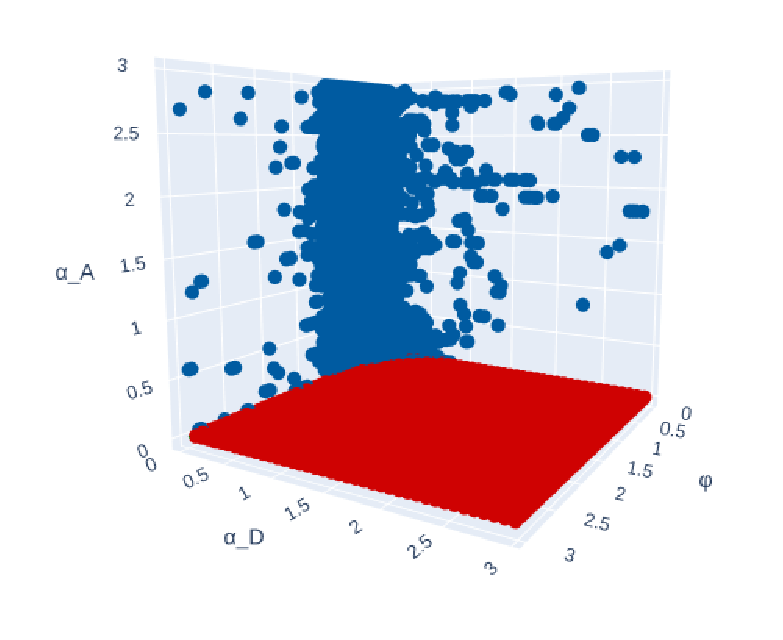
\includegraphics[width=0.9\linewidth]{figs/approx_surface_decision_space.eps}
    \caption{Decision space for FlipIt with IE with approximated BRDVs for the defender plotted in blue and the ones for the attacker in red.}
    \label{fig:approx_surface}
\end{figure}

Regardless the shape of the these geometric figures, since by definition each PSNE is a state in which all players play a BRDV simultaneously, we can think about the PSNEs as the intersections of the figures for all players.
This concept has been explictly used for single-objective players in \cite{dijk2013flipit}, and implictly in the GA implementation by \cite{sherfield2018flipthem}, but to the best of our knowledge, it has not been generalized to multi-objective players or multi-player games until now.


\subsection{Numerical approximation procedure}

The problem with the idealized procedure is that in digital computers it is not feasible to run infinite independent multi-objective optimizations.
On a lesser note, each optimization is also not perfectly continuous since even ``real'' variables are represented with a finite number of bits in a computer, although for all practical purposes we can consider them ``real'' valued.

To address these limitations while still confirming the theoretical foundations of the idealized procedure, we propose a numerical procedure that discretizes the OSPs for each player, then approximates the BRDVs for each OSP by means of a regular multi-objective evolutionary algorithm.
With this, we aim to avoid game-theoretical-specific fitness functions (see \cite{leite2024cec} \cite{lung2008computing} \cite{lung2020pareto}), adopting a Pareto-Front approach instead that shall appear more intuitive to researchers in the field of computational optimization.
The PSNEs are then computed as the points from each player which are less than a small arbitrary distance $\epsilon$ apart of a point from every other player (i.e., the intersection of the approximated BRDVs).



\section{Experimental setup}
\label{methodology}

NSGA-II was arbitrarily chosen as the multi-objective evolutionary algorithm for each BRDV approximation, even though the BRDVs for the attacker are actually single-objective problems.
This was done to keep the experimental code short and simple, even though a single-objective algorithm could (and arguably should) be especially allocated for single-objective players.


\section{Results and discussion}
\label{results}


\section{Conclusions and future works}
\label{conclusions}

TBD

\bibliographystyle{plain}
\bibliography{symposium}

%------------------------------------------------------------------------------
\end{document}
